% Options for packages loaded elsewhere
\PassOptionsToPackage{unicode}{hyperref}
\PassOptionsToPackage{hyphens}{url}
%
\documentclass[
]{article}
\usepackage{amsmath,amssymb}
\usepackage{iftex}
\ifPDFTeX
  \usepackage[T1]{fontenc}
  \usepackage[utf8]{inputenc}
  \usepackage{textcomp} % provide euro and other symbols
\else % if luatex or xetex
  \usepackage{unicode-math} % this also loads fontspec
  \defaultfontfeatures{Scale=MatchLowercase}
  \defaultfontfeatures[\rmfamily]{Ligatures=TeX,Scale=1}
\fi
\usepackage{lmodern}
\ifPDFTeX\else
  % xetex/luatex font selection
\fi
% Use upquote if available, for straight quotes in verbatim environments
\IfFileExists{upquote.sty}{\usepackage{upquote}}{}
\IfFileExists{microtype.sty}{% use microtype if available
  \usepackage[]{microtype}
  \UseMicrotypeSet[protrusion]{basicmath} % disable protrusion for tt fonts
}{}
\makeatletter
\@ifundefined{KOMAClassName}{% if non-KOMA class
  \IfFileExists{parskip.sty}{%
    \usepackage{parskip}
  }{% else
    \setlength{\parindent}{0pt}
    \setlength{\parskip}{6pt plus 2pt minus 1pt}}
}{% if KOMA class
  \KOMAoptions{parskip=half}}
\makeatother
\usepackage{xcolor}
\usepackage[margin=1in]{geometry}
\usepackage{color}
\usepackage{fancyvrb}
\newcommand{\VerbBar}{|}
\newcommand{\VERB}{\Verb[commandchars=\\\{\}]}
\DefineVerbatimEnvironment{Highlighting}{Verbatim}{commandchars=\\\{\}}
% Add ',fontsize=\small' for more characters per line
\usepackage{framed}
\definecolor{shadecolor}{RGB}{248,248,248}
\newenvironment{Shaded}{\begin{snugshade}}{\end{snugshade}}
\newcommand{\AlertTok}[1]{\textcolor[rgb]{0.94,0.16,0.16}{#1}}
\newcommand{\AnnotationTok}[1]{\textcolor[rgb]{0.56,0.35,0.01}{\textbf{\textit{#1}}}}
\newcommand{\AttributeTok}[1]{\textcolor[rgb]{0.13,0.29,0.53}{#1}}
\newcommand{\BaseNTok}[1]{\textcolor[rgb]{0.00,0.00,0.81}{#1}}
\newcommand{\BuiltInTok}[1]{#1}
\newcommand{\CharTok}[1]{\textcolor[rgb]{0.31,0.60,0.02}{#1}}
\newcommand{\CommentTok}[1]{\textcolor[rgb]{0.56,0.35,0.01}{\textit{#1}}}
\newcommand{\CommentVarTok}[1]{\textcolor[rgb]{0.56,0.35,0.01}{\textbf{\textit{#1}}}}
\newcommand{\ConstantTok}[1]{\textcolor[rgb]{0.56,0.35,0.01}{#1}}
\newcommand{\ControlFlowTok}[1]{\textcolor[rgb]{0.13,0.29,0.53}{\textbf{#1}}}
\newcommand{\DataTypeTok}[1]{\textcolor[rgb]{0.13,0.29,0.53}{#1}}
\newcommand{\DecValTok}[1]{\textcolor[rgb]{0.00,0.00,0.81}{#1}}
\newcommand{\DocumentationTok}[1]{\textcolor[rgb]{0.56,0.35,0.01}{\textbf{\textit{#1}}}}
\newcommand{\ErrorTok}[1]{\textcolor[rgb]{0.64,0.00,0.00}{\textbf{#1}}}
\newcommand{\ExtensionTok}[1]{#1}
\newcommand{\FloatTok}[1]{\textcolor[rgb]{0.00,0.00,0.81}{#1}}
\newcommand{\FunctionTok}[1]{\textcolor[rgb]{0.13,0.29,0.53}{\textbf{#1}}}
\newcommand{\ImportTok}[1]{#1}
\newcommand{\InformationTok}[1]{\textcolor[rgb]{0.56,0.35,0.01}{\textbf{\textit{#1}}}}
\newcommand{\KeywordTok}[1]{\textcolor[rgb]{0.13,0.29,0.53}{\textbf{#1}}}
\newcommand{\NormalTok}[1]{#1}
\newcommand{\OperatorTok}[1]{\textcolor[rgb]{0.81,0.36,0.00}{\textbf{#1}}}
\newcommand{\OtherTok}[1]{\textcolor[rgb]{0.56,0.35,0.01}{#1}}
\newcommand{\PreprocessorTok}[1]{\textcolor[rgb]{0.56,0.35,0.01}{\textit{#1}}}
\newcommand{\RegionMarkerTok}[1]{#1}
\newcommand{\SpecialCharTok}[1]{\textcolor[rgb]{0.81,0.36,0.00}{\textbf{#1}}}
\newcommand{\SpecialStringTok}[1]{\textcolor[rgb]{0.31,0.60,0.02}{#1}}
\newcommand{\StringTok}[1]{\textcolor[rgb]{0.31,0.60,0.02}{#1}}
\newcommand{\VariableTok}[1]{\textcolor[rgb]{0.00,0.00,0.00}{#1}}
\newcommand{\VerbatimStringTok}[1]{\textcolor[rgb]{0.31,0.60,0.02}{#1}}
\newcommand{\WarningTok}[1]{\textcolor[rgb]{0.56,0.35,0.01}{\textbf{\textit{#1}}}}
\usepackage{graphicx}
\makeatletter
\def\maxwidth{\ifdim\Gin@nat@width>\linewidth\linewidth\else\Gin@nat@width\fi}
\def\maxheight{\ifdim\Gin@nat@height>\textheight\textheight\else\Gin@nat@height\fi}
\makeatother
% Scale images if necessary, so that they will not overflow the page
% margins by default, and it is still possible to overwrite the defaults
% using explicit options in \includegraphics[width, height, ...]{}
\setkeys{Gin}{width=\maxwidth,height=\maxheight,keepaspectratio}
% Set default figure placement to htbp
\makeatletter
\def\fps@figure{htbp}
\makeatother
\setlength{\emergencystretch}{3em} % prevent overfull lines
\providecommand{\tightlist}{%
  \setlength{\itemsep}{0pt}\setlength{\parskip}{0pt}}
\setcounter{secnumdepth}{-\maxdimen} % remove section numbering
\usepackage{float}
\usepackage{tabularray}
\usepackage[normalem]{ulem}
\usepackage{graphicx}
\UseTblrLibrary{booktabs}
\UseTblrLibrary{rotating}
\UseTblrLibrary{siunitx}
\NewTableCommand{\tinytableDefineColor}[3]{\definecolor{#1}{#2}{#3}}
\newcommand{\tinytableTabularrayUnderline}[1]{\underline{#1}}
\newcommand{\tinytableTabularrayStrikeout}[1]{\sout{#1}}
\ifLuaTeX
  \usepackage{selnolig}  % disable illegal ligatures
\fi
\usepackage{bookmark}
\IfFileExists{xurl.sty}{\usepackage{xurl}}{} % add URL line breaks if available
\urlstyle{same}
\hypersetup{
  pdftitle={State-of-Life-Predicting-Life-Expectancy-from-1970s-Census-Data},
  pdfauthor={XunSun},
  hidelinks,
  pdfcreator={LaTeX via pandoc}}

\title{State-of-Life-Predicting-Life-Expectancy-from-1970s-Census-Data}
\author{XunSun}
\date{2024-12-14}

\begin{document}
\maketitle

\begin{Shaded}
\begin{Highlighting}[]
\FunctionTok{library}\NormalTok{(tidyverse)}
\end{Highlighting}
\end{Shaded}

\begin{verbatim}
## -- Attaching core tidyverse packages ------------------------ tidyverse 2.0.0 --
## v dplyr     1.1.4     v readr     2.1.5
## v forcats   1.0.0     v stringr   1.5.1
## v ggplot2   3.5.1     v tibble    3.2.1
## v lubridate 1.9.3     v tidyr     1.3.1
## v purrr     1.0.2     
## -- Conflicts ------------------------------------------ tidyverse_conflicts() --
## x dplyr::filter() masks stats::filter()
## x dplyr::lag()    masks stats::lag()
## i Use the conflicted package (<http://conflicted.r-lib.org/>) to force all conflicts to become errors
\end{verbatim}

\begin{Shaded}
\begin{Highlighting}[]
\FunctionTok{library}\NormalTok{(GGally)}
\end{Highlighting}
\end{Shaded}

\begin{verbatim}
## Warning: 程序包'GGally'是用R版本4.4.2 来建造的
\end{verbatim}

\begin{verbatim}
## Registered S3 method overwritten by 'GGally':
##   method from   
##   +.gg   ggplot2
\end{verbatim}

\begin{Shaded}
\begin{Highlighting}[]
\FunctionTok{library}\NormalTok{(patchwork)}
\FunctionTok{library}\NormalTok{(gt)}
\end{Highlighting}
\end{Shaded}

\begin{verbatim}
## Warning: 程序包'gt'是用R版本4.4.2 来建造的
\end{verbatim}

\begin{Shaded}
\begin{Highlighting}[]
\FunctionTok{library}\NormalTok{(leaps)}
\end{Highlighting}
\end{Shaded}

\begin{verbatim}
## Warning: 程序包'leaps'是用R版本4.4.2 来建造的
\end{verbatim}

\begin{Shaded}
\begin{Highlighting}[]
\FunctionTok{library}\NormalTok{(caret)}
\end{Highlighting}
\end{Shaded}

\begin{verbatim}
## Warning: 程序包'caret'是用R版本4.4.2 来建造的
\end{verbatim}

\begin{verbatim}
## 载入需要的程序包:lattice
## 
## 载入程序包:'caret'
## 
## The following object is masked from 'package:purrr':
## 
##     lift
\end{verbatim}

\begin{Shaded}
\begin{Highlighting}[]
\FunctionTok{library}\NormalTok{(ggplot2)}
\FunctionTok{library}\NormalTok{(dbplyr)}
\end{Highlighting}
\end{Shaded}

\begin{verbatim}
## 
## 载入程序包:'dbplyr'
## 
## The following objects are masked from 'package:dplyr':
## 
##     ident, sql
\end{verbatim}

R dataset state.x77 from library(faraway) contains information on 50
states from 1970s collected by US Census Bureau. The goal is to predict
`life expectancy' using a combination of remaining variables.

\begin{Shaded}
\begin{Highlighting}[]
\FunctionTok{library}\NormalTok{(faraway)}
\end{Highlighting}
\end{Shaded}

\begin{verbatim}
## Warning: 程序包'faraway'是用R版本4.4.2 来建造的
\end{verbatim}

\begin{verbatim}
## 
## 载入程序包:'faraway'
\end{verbatim}

\begin{verbatim}
## The following object is masked from 'package:lattice':
## 
##     melanoma
\end{verbatim}

\begin{verbatim}
## The following object is masked from 'package:GGally':
## 
##     happy
\end{verbatim}

\begin{Shaded}
\begin{Highlighting}[]
\NormalTok{data.state }\OtherTok{\textless{}{-}} \FunctionTok{as.data.frame}\NormalTok{(state.x77)}\SpecialCharTok{|\textgreater{}} 
\NormalTok{  janitor}\SpecialCharTok{::}\FunctionTok{clean\_names}\NormalTok{() }
\FunctionTok{head}\NormalTok{(data.state)}
\end{Highlighting}
\end{Shaded}

\begin{verbatim}
##            population income illiteracy life_exp murder hs_grad frost   area
## Alabama          3615   3624        2.1    69.05   15.1    41.3    20  50708
## Alaska            365   6315        1.5    69.31   11.3    66.7   152 566432
## Arizona          2212   4530        1.8    70.55    7.8    58.1    15 113417
## Arkansas         2110   3378        1.9    70.66   10.1    39.9    65  51945
## California      21198   5114        1.1    71.71   10.3    62.6    20 156361
## Colorado         2541   4884        0.7    72.06    6.8    63.9   166 103766
\end{verbatim}

\begin{Shaded}
\begin{Highlighting}[]
\FunctionTok{view}\NormalTok{(data.state)}
\end{Highlighting}
\end{Shaded}

\begin{enumerate}
\def\labelenumi{\alph{enumi})}
\tightlist
\item
  Provide descriptive statistics for all variables of interest -- no
  test required
\end{enumerate}

\begin{Shaded}
\begin{Highlighting}[]
\FunctionTok{summary}\NormalTok{(data.state)}
\end{Highlighting}
\end{Shaded}

\begin{verbatim}
##    population        income       illiteracy       life_exp    
##  Min.   :  365   Min.   :3098   Min.   :0.500   Min.   :67.96  
##  1st Qu.: 1080   1st Qu.:3993   1st Qu.:0.625   1st Qu.:70.12  
##  Median : 2838   Median :4519   Median :0.950   Median :70.67  
##  Mean   : 4246   Mean   :4436   Mean   :1.170   Mean   :70.88  
##  3rd Qu.: 4968   3rd Qu.:4814   3rd Qu.:1.575   3rd Qu.:71.89  
##  Max.   :21198   Max.   :6315   Max.   :2.800   Max.   :73.60  
##      murder          hs_grad          frost             area       
##  Min.   : 1.400   Min.   :37.80   Min.   :  0.00   Min.   :  1049  
##  1st Qu.: 4.350   1st Qu.:48.05   1st Qu.: 66.25   1st Qu.: 36985  
##  Median : 6.850   Median :53.25   Median :114.50   Median : 54277  
##  Mean   : 7.378   Mean   :53.11   Mean   :104.46   Mean   : 70736  
##  3rd Qu.:10.675   3rd Qu.:59.15   3rd Qu.:139.75   3rd Qu.: 81163  
##  Max.   :15.100   Max.   :67.30   Max.   :188.00   Max.   :566432
\end{verbatim}

Examine exploratory plots, e.g., scatter plots, histograms, boxplots to
get a sense of the data and possible variable transformations.

\begin{Shaded}
\begin{Highlighting}[]
\NormalTok{data.state }\SpecialCharTok{|\textgreater{}}
  \FunctionTok{relocate}\NormalTok{(}\StringTok{\textasciigrave{}}\AttributeTok{life\_exp}\StringTok{\textasciigrave{}}\NormalTok{) }\SpecialCharTok{|\textgreater{}}
  \FunctionTok{ggpairs}\NormalTok{()}
\end{Highlighting}
\end{Shaded}

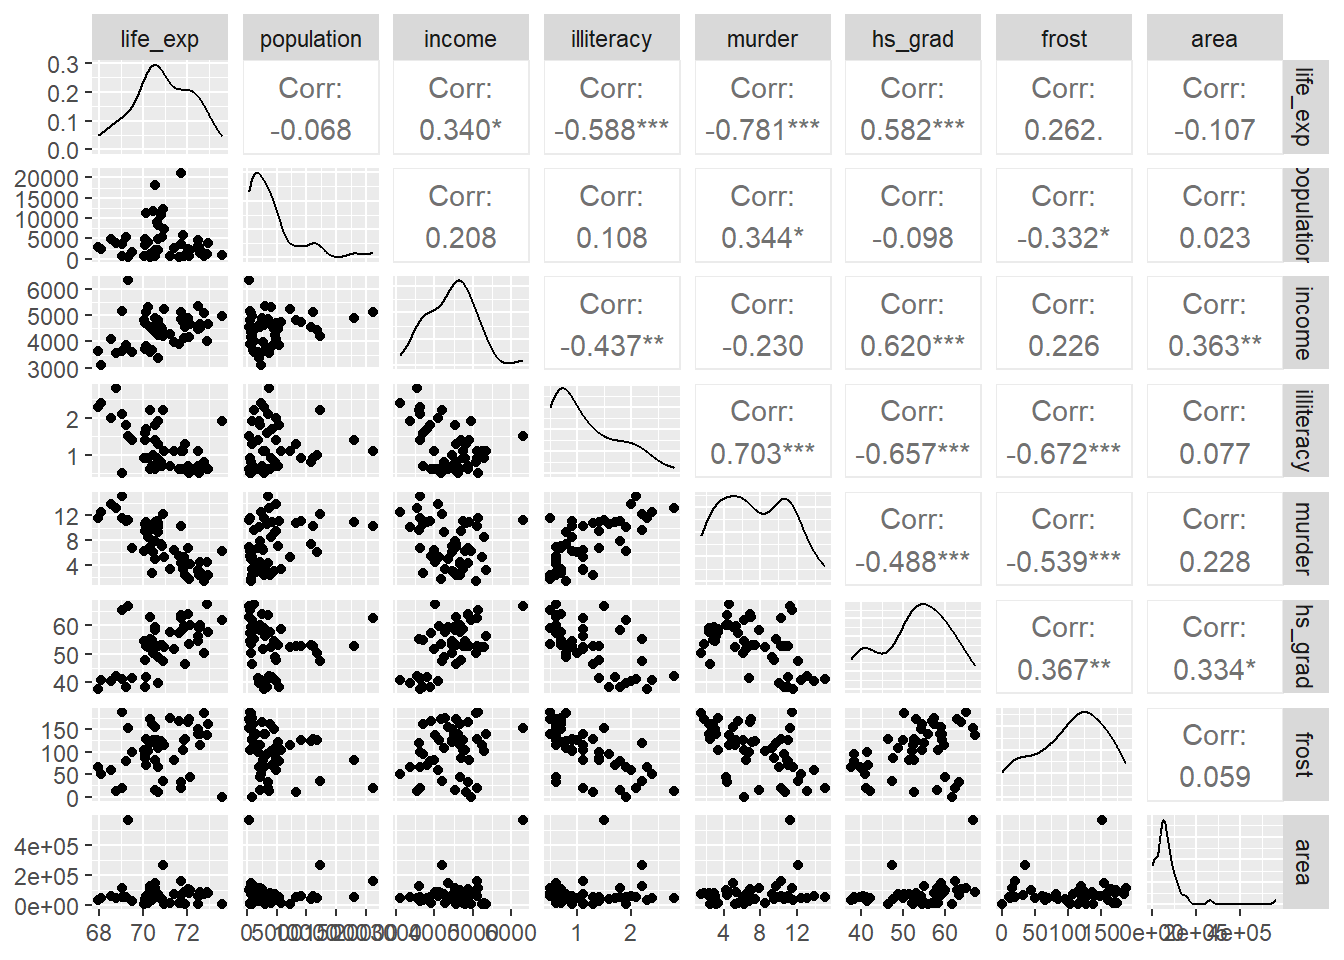
\includegraphics{State-of-Life-Predicting-Life-Expectancy-from-1970s-Census-Data_files/figure-latex/unnamed-chunk-4-1.pdf}
\#\# look for appropriate transformations

\begin{Shaded}
\begin{Highlighting}[]
\NormalTok{density\_plot\_population }\OtherTok{\textless{}{-}}\NormalTok{data.state }\SpecialCharTok{|\textgreater{}}
  \FunctionTok{ggplot}\NormalTok{(}\FunctionTok{aes}\NormalTok{(}\AttributeTok{x =}\NormalTok{ population)) }\SpecialCharTok{+}
  \FunctionTok{geom\_density}\NormalTok{()}

\NormalTok{density\_plot\_logpopulation }\OtherTok{\textless{}{-}}\NormalTok{data.state }\SpecialCharTok{|\textgreater{}}
  \FunctionTok{mutate}\NormalTok{(}\AttributeTok{log\_population =} \FunctionTok{log}\NormalTok{(population)) }\SpecialCharTok{|\textgreater{}}
  \FunctionTok{ggplot}\NormalTok{(}\FunctionTok{aes}\NormalTok{(}\AttributeTok{x =}\NormalTok{ log\_population)) }\SpecialCharTok{+} \FunctionTok{geom\_density}\NormalTok{()}

\NormalTok{density\_plot\_inver\_population }\OtherTok{\textless{}{-}}\NormalTok{data.state }\SpecialCharTok{|\textgreater{}}
  \FunctionTok{mutate}\NormalTok{(}\AttributeTok{inver\_population =} \DecValTok{1}\SpecialCharTok{/}\NormalTok{(population)) }\SpecialCharTok{|\textgreater{}}
  \FunctionTok{ggplot}\NormalTok{(}\FunctionTok{aes}\NormalTok{(}\AttributeTok{x =}\NormalTok{ inver\_population)) }\SpecialCharTok{+} \FunctionTok{geom\_density}\NormalTok{()}


\NormalTok{density\_plot\_population }\SpecialCharTok{+}\NormalTok{ density\_plot\_logpopulation }\SpecialCharTok{+}\NormalTok{ density\_plot\_inver\_population}
\end{Highlighting}
\end{Shaded}

\includegraphics{State-of-Life-Predicting-Life-Expectancy-from-1970s-Census-Data_files/figure-latex/unnamed-chunk-5-1.pdf}

\begin{Shaded}
\begin{Highlighting}[]
\NormalTok{density\_plot\_area }\OtherTok{\textless{}{-}}\NormalTok{ data.state }\SpecialCharTok{|\textgreater{}}
  \FunctionTok{ggplot}\NormalTok{(}\FunctionTok{aes}\NormalTok{(}\AttributeTok{x =}\NormalTok{ area)) }\SpecialCharTok{+}
  \FunctionTok{geom\_density}\NormalTok{()}

\NormalTok{density\_plot\_logarea }\OtherTok{\textless{}{-}}\NormalTok{ data.state }\SpecialCharTok{|\textgreater{}}
  \FunctionTok{mutate}\NormalTok{(}\AttributeTok{log\_area =} \FunctionTok{log}\NormalTok{(area)) }\SpecialCharTok{|\textgreater{}}
  \FunctionTok{ggplot}\NormalTok{(}\FunctionTok{aes}\NormalTok{(}\AttributeTok{x =}\NormalTok{ log\_area)) }\SpecialCharTok{+} \FunctionTok{geom\_density}\NormalTok{()}

\NormalTok{density\_plot\_area }\SpecialCharTok{+}\NormalTok{ density\_plot\_logarea}
\end{Highlighting}
\end{Shaded}

\includegraphics{State-of-Life-Predicting-Life-Expectancy-from-1970s-Census-Data_files/figure-latex/unnamed-chunk-6-1.pdf}

\begin{Shaded}
\begin{Highlighting}[]
\NormalTok{density\_plot\_illiteracy }\OtherTok{\textless{}{-}}\NormalTok{ data.state }\SpecialCharTok{|\textgreater{}}
  \FunctionTok{ggplot}\NormalTok{(}\FunctionTok{aes}\NormalTok{(}\AttributeTok{x =}\NormalTok{ illiteracy)) }\SpecialCharTok{+}
  \FunctionTok{geom\_density}\NormalTok{()}

\NormalTok{density\_plot\_logilliteracy }\OtherTok{\textless{}{-}}\NormalTok{ data.state }\SpecialCharTok{|\textgreater{}}
  \FunctionTok{mutate}\NormalTok{(}\AttributeTok{log\_illiteracy =} \FunctionTok{log}\NormalTok{(illiteracy)) }\SpecialCharTok{|\textgreater{}}
  \FunctionTok{ggplot}\NormalTok{(}\FunctionTok{aes}\NormalTok{(}\AttributeTok{x =}\NormalTok{ log\_illiteracy)) }\SpecialCharTok{+} \FunctionTok{geom\_density}\NormalTok{()}

\NormalTok{density\_plot\_illiteracy }\SpecialCharTok{+}\NormalTok{ density\_plot\_logilliteracy}
\end{Highlighting}
\end{Shaded}

\includegraphics{State-of-Life-Predicting-Life-Expectancy-from-1970s-Census-Data_files/figure-latex/unnamed-chunk-7-1.pdf}

\begin{Shaded}
\begin{Highlighting}[]
\NormalTok{qq\_population }\OtherTok{\textless{}{-}}\NormalTok{ data.state }\SpecialCharTok{|\textgreater{}}
  \FunctionTok{ggplot}\NormalTok{(}\FunctionTok{aes}\NormalTok{(}\AttributeTok{sample =}\NormalTok{ population)) }\SpecialCharTok{+}
  \FunctionTok{stat\_qq}\NormalTok{() }\SpecialCharTok{+}
  \FunctionTok{stat\_qq\_line}\NormalTok{() }\SpecialCharTok{+}
  \FunctionTok{ggtitle}\NormalTok{(}\StringTok{"QQ Plot: Population"}\NormalTok{)}

\NormalTok{qq\_log\_population }\OtherTok{\textless{}{-}}\NormalTok{ data.state }\SpecialCharTok{|\textgreater{}}
  \FunctionTok{mutate}\NormalTok{(}\AttributeTok{log\_population =} \FunctionTok{log}\NormalTok{(population)) }\SpecialCharTok{|\textgreater{}}
  \FunctionTok{ggplot}\NormalTok{(}\FunctionTok{aes}\NormalTok{(}\AttributeTok{sample =}\NormalTok{ log\_population)) }\SpecialCharTok{+}
  \FunctionTok{stat\_qq}\NormalTok{() }\SpecialCharTok{+}
  \FunctionTok{stat\_qq\_line}\NormalTok{() }\SpecialCharTok{+}
  \FunctionTok{ggtitle}\NormalTok{(}\StringTok{"QQ Plot: Log Population"}\NormalTok{)}

\NormalTok{qq\_inver\_population }\OtherTok{\textless{}{-}}\NormalTok{ data.state }\SpecialCharTok{|\textgreater{}}
  \FunctionTok{mutate}\NormalTok{(}\AttributeTok{inver\_population =} \DecValTok{1} \SpecialCharTok{/}\NormalTok{ (population)) }\SpecialCharTok{|\textgreater{}}
  \FunctionTok{ggplot}\NormalTok{(}\FunctionTok{aes}\NormalTok{(}\AttributeTok{sample =}\NormalTok{ inver\_population)) }\SpecialCharTok{+}
  \FunctionTok{stat\_qq}\NormalTok{() }\SpecialCharTok{+}
  \FunctionTok{stat\_qq\_line}\NormalTok{() }\SpecialCharTok{+}
  \FunctionTok{ggtitle}\NormalTok{(}\StringTok{"QQ Plot: Inverse Population"}\NormalTok{)}

\CommentTok{\# QQ Plots for Area}
\NormalTok{qq\_area }\OtherTok{\textless{}{-}}\NormalTok{ data.state }\SpecialCharTok{|\textgreater{}}
  \FunctionTok{ggplot}\NormalTok{(}\FunctionTok{aes}\NormalTok{(}\AttributeTok{sample =}\NormalTok{ area)) }\SpecialCharTok{+}
  \FunctionTok{stat\_qq}\NormalTok{() }\SpecialCharTok{+}
  \FunctionTok{stat\_qq\_line}\NormalTok{() }\SpecialCharTok{+}
  \FunctionTok{ggtitle}\NormalTok{(}\StringTok{"QQ Plot: Area"}\NormalTok{)}

\NormalTok{qq\_log\_area }\OtherTok{\textless{}{-}}\NormalTok{ data.state }\SpecialCharTok{|\textgreater{}}
  \FunctionTok{mutate}\NormalTok{(}\AttributeTok{log\_area =} \FunctionTok{log}\NormalTok{(area)) }\SpecialCharTok{|\textgreater{}}
  \FunctionTok{ggplot}\NormalTok{(}\FunctionTok{aes}\NormalTok{(}\AttributeTok{sample =}\NormalTok{ log\_area)) }\SpecialCharTok{+}
  \FunctionTok{stat\_qq}\NormalTok{() }\SpecialCharTok{+}
  \FunctionTok{stat\_qq\_line}\NormalTok{() }\SpecialCharTok{+}
  \FunctionTok{ggtitle}\NormalTok{(}\StringTok{"QQ Plot: Log Area"}\NormalTok{)}

\CommentTok{\# QQ Plots for Illiteracy}
\NormalTok{qq\_illiteracy }\OtherTok{\textless{}{-}}\NormalTok{ data.state }\SpecialCharTok{|\textgreater{}}
  \FunctionTok{ggplot}\NormalTok{(}\FunctionTok{aes}\NormalTok{(}\AttributeTok{sample =}\NormalTok{ illiteracy)) }\SpecialCharTok{+}
  \FunctionTok{stat\_qq}\NormalTok{() }\SpecialCharTok{+}
  \FunctionTok{stat\_qq\_line}\NormalTok{() }\SpecialCharTok{+}
  \FunctionTok{ggtitle}\NormalTok{(}\StringTok{"QQ Plot: Illiteracy"}\NormalTok{)}

\NormalTok{qq\_log\_illiteracy }\OtherTok{\textless{}{-}}\NormalTok{ data.state }\SpecialCharTok{|\textgreater{}}
  \FunctionTok{mutate}\NormalTok{(}\AttributeTok{log\_illiteracy =} \FunctionTok{log}\NormalTok{(illiteracy)) }\SpecialCharTok{|\textgreater{}}
  \FunctionTok{ggplot}\NormalTok{(}\FunctionTok{aes}\NormalTok{(}\AttributeTok{sample =}\NormalTok{ log\_illiteracy)) }\SpecialCharTok{+}
  \FunctionTok{stat\_qq}\NormalTok{() }\SpecialCharTok{+}
  \FunctionTok{stat\_qq\_line}\NormalTok{() }\SpecialCharTok{+}
  \FunctionTok{ggtitle}\NormalTok{(}\StringTok{"QQ Plot: Log Illiteracy"}\NormalTok{)}

\CommentTok{\# Combine QQ Plots with Patchwork for Comparison}
\FunctionTok{library}\NormalTok{(patchwork)}

\NormalTok{(qq\_population }\SpecialCharTok{|}\NormalTok{ qq\_log\_population }\SpecialCharTok{|}\NormalTok{ qq\_inver\_population) }\SpecialCharTok{/} 
\NormalTok{(qq\_area }\SpecialCharTok{|}\NormalTok{ qq\_log\_area) }\SpecialCharTok{/} 
\NormalTok{(qq\_illiteracy }\SpecialCharTok{|}\NormalTok{ qq\_log\_illiteracy)}
\end{Highlighting}
\end{Shaded}

\includegraphics{State-of-Life-Predicting-Life-Expectancy-from-1970s-Census-Data_files/figure-latex/unnamed-chunk-8-1.pdf}

\begin{Shaded}
\begin{Highlighting}[]
\NormalTok{data.state }\OtherTok{\textless{}{-}}\NormalTok{ data.state }\SpecialCharTok{|\textgreater{}}
  \FunctionTok{mutate}\NormalTok{(}\AttributeTok{log\_Population =} \FunctionTok{log}\NormalTok{(population)) }\SpecialCharTok{|\textgreater{}}
  \FunctionTok{select}\NormalTok{(}\SpecialCharTok{{-}}\NormalTok{population)}
\FunctionTok{view}\NormalTok{(data.state)}
\end{Highlighting}
\end{Shaded}

\begin{Shaded}
\begin{Highlighting}[]
\CommentTok{\# Define the response variable and dataset}
\NormalTok{response }\OtherTok{\textless{}{-}} \StringTok{"life\_expectancy"}  \CommentTok{\# Replace with your actual response variable}
\NormalTok{data }\OtherTok{\textless{}{-}}\NormalTok{ data.state            }\CommentTok{\# Your dataset}

\CommentTok{\# Null model}
\NormalTok{null\_model }\OtherTok{\textless{}{-}} \FunctionTok{lm}\NormalTok{(life\_exp }\SpecialCharTok{\textasciitilde{}} \DecValTok{1}\NormalTok{, }\AttributeTok{data =}\NormalTok{ data)}

\CommentTok{\# Full model (all predictors)}
\NormalTok{full\_model }\OtherTok{\textless{}{-}} \FunctionTok{lm}\NormalTok{(life\_exp }\SpecialCharTok{\textasciitilde{}}\NormalTok{ ., }\AttributeTok{data =}\NormalTok{ data)}
\end{Highlighting}
\end{Shaded}

\begin{Shaded}
\begin{Highlighting}[]
\FunctionTok{library}\NormalTok{(MASS)}
\end{Highlighting}
\end{Shaded}

\begin{verbatim}
## Warning: 程序包'MASS'是用R版本4.4.2 来建造的
\end{verbatim}

\begin{verbatim}
## 
## 载入程序包:'MASS'
\end{verbatim}

\begin{verbatim}
## The following object is masked from 'package:patchwork':
## 
##     area
\end{verbatim}

\begin{verbatim}
## The following object is masked from 'package:dplyr':
## 
##     select
\end{verbatim}

\begin{Shaded}
\begin{Highlighting}[]
\FunctionTok{library}\NormalTok{(olsrr)}
\end{Highlighting}
\end{Shaded}

\begin{verbatim}
## Warning: 程序包'olsrr'是用R版本4.4.2 来建造的
\end{verbatim}

\begin{verbatim}
## 
## 载入程序包:'olsrr'
\end{verbatim}

\begin{verbatim}
## The following object is masked from 'package:MASS':
## 
##     cement
\end{verbatim}

\begin{verbatim}
## The following object is masked from 'package:faraway':
## 
##     hsb
\end{verbatim}

\begin{verbatim}
## The following object is masked from 'package:datasets':
## 
##     rivers
\end{verbatim}

\begin{Shaded}
\begin{Highlighting}[]
\CommentTok{\# Forward Selection}
\NormalTok{forward\_aic }\OtherTok{\textless{}{-}} \FunctionTok{stepAIC}\NormalTok{(null\_model, }
                         \AttributeTok{scope =} \FunctionTok{list}\NormalTok{(}\AttributeTok{lower =}\NormalTok{ null\_model, }\AttributeTok{upper =}\NormalTok{ full\_model), }\AttributeTok{direction =} \StringTok{"forward"}\NormalTok{)}
\end{Highlighting}
\end{Shaded}

\begin{verbatim}
## Start:  AIC=30.44
## life_exp ~ 1
## 
##                  Df Sum of Sq    RSS     AIC
## + murder          1    53.838 34.461 -14.609
## + illiteracy      1    30.578 57.721  11.179
## + hs_grad         1    29.931 58.368  11.737
## + income          1    10.223 78.076  26.283
## + frost           1     6.064 82.235  28.878
## <none>                        88.299  30.435
## + log_Population  1     1.054 87.245  31.835
## + area            1     1.017 87.282  31.856
## 
## Step:  AIC=-14.61
## life_exp ~ murder
## 
##                  Df Sum of Sq    RSS     AIC
## + hs_grad         1    4.6910 29.770 -19.925
## + frost           1    3.1346 31.327 -17.378
## + log_Population  1    2.9854 31.476 -17.140
## + income          1    2.4047 32.057 -16.226
## <none>                        34.461 -14.609
## + area            1    0.4697 33.992 -13.295
## + illiteracy      1    0.2732 34.188 -13.007
## 
## Step:  AIC=-19.93
## life_exp ~ murder + hs_grad
## 
##                  Df Sum of Sq    RSS     AIC
## + log_Population  1    4.6350 25.135 -26.387
## + frost           1    4.3987 25.372 -25.920
## <none>                        29.770 -19.925
## + illiteracy      1    0.4419 29.328 -18.673
## + area            1    0.2775 29.493 -18.394
## + income          1    0.1022 29.668 -18.097
## 
## Step:  AIC=-26.39
## life_exp ~ murder + hs_grad + log_Population
## 
##              Df Sum of Sq    RSS     AIC
## + frost       1   2.21416 22.921 -28.998
## + illiteracy  1   1.10754 24.028 -26.640
## <none>                    25.135 -26.387
## + income      1   0.11819 25.017 -24.623
## + area        1   0.00175 25.134 -24.391
## 
## Step:  AIC=-29
## life_exp ~ murder + hs_grad + log_Population + frost
## 
##              Df Sum of Sq    RSS     AIC
## <none>                    22.921 -28.998
## + illiteracy  1  0.051595 22.870 -27.111
## + area        1  0.015956 22.905 -27.033
## + income      1  0.010673 22.911 -27.021
\end{verbatim}

\begin{Shaded}
\begin{Highlighting}[]
\CommentTok{\# Summary of the selected model}
\FunctionTok{summary}\NormalTok{(forward\_aic)}
\end{Highlighting}
\end{Shaded}

\begin{verbatim}
## 
## Call:
## lm(formula = life_exp ~ murder + hs_grad + log_Population + frost, 
##     data = data)
## 
## Residuals:
##      Min       1Q   Median       3Q      Max 
## -1.41760 -0.43880  0.02539  0.52066  1.63048 
## 
## Coefficients:
##                 Estimate Std. Error t value Pr(>|t|)    
## (Intercept)    68.720810   1.416828  48.503  < 2e-16 ***
## murder         -0.290016   0.035440  -8.183 1.87e-10 ***
## hs_grad         0.054550   0.014758   3.696 0.000591 ***
## log_Population  0.246836   0.112539   2.193 0.033491 *  
## frost          -0.005174   0.002482  -2.085 0.042779 *  
## ---
## Signif. codes:  0 '***' 0.001 '**' 0.01 '*' 0.05 '.' 0.1 ' ' 1
## 
## Residual standard error: 0.7137 on 45 degrees of freedom
## Multiple R-squared:  0.7404, Adjusted R-squared:  0.7173 
## F-statistic: 32.09 on 4 and 45 DF,  p-value: 1.17e-12
\end{verbatim}

\begin{Shaded}
\begin{Highlighting}[]
\NormalTok{n }\OtherTok{\textless{}{-}} \FunctionTok{nrow}\NormalTok{(data.state) }
\NormalTok{forward\_bic }\OtherTok{\textless{}{-}} \FunctionTok{step}\NormalTok{(null\_model, }
                    \AttributeTok{scope =} \FunctionTok{list}\NormalTok{(}\AttributeTok{lower =}\NormalTok{ null\_model, }\AttributeTok{upper =}\NormalTok{ full\_model), }
                    \AttributeTok{direction =} \StringTok{"forward"}\NormalTok{, }
                    \AttributeTok{k =} \FunctionTok{log}\NormalTok{(n)) }
\end{Highlighting}
\end{Shaded}

\begin{verbatim}
## Start:  AIC=32.35
## life_exp ~ 1
## 
##                  Df Sum of Sq    RSS     AIC
## + murder          1    53.838 34.461 -10.785
## + illiteracy      1    30.578 57.721  15.004
## + hs_grad         1    29.931 58.368  15.561
## + income          1    10.223 78.076  30.107
## <none>                        88.299  32.347
## + frost           1     6.064 82.235  32.702
## + log_Population  1     1.054 87.245  35.659
## + area            1     1.017 87.282  35.680
## 
## Step:  AIC=-10.79
## life_exp ~ murder
## 
##                  Df Sum of Sq    RSS      AIC
## + hs_grad         1    4.6910 29.770 -14.1894
## + frost           1    3.1346 31.327 -11.6415
## + log_Population  1    2.9854 31.476 -11.4039
## <none>                        34.461 -10.7852
## + income          1    2.4047 32.057 -10.4900
## + area            1    0.4697 33.992  -7.5593
## + illiteracy      1    0.2732 34.188  -7.2712
## 
## Step:  AIC=-14.19
## life_exp ~ murder + hs_grad
## 
##                  Df Sum of Sq    RSS     AIC
## + log_Population  1    4.6350 25.135 -18.739
## + frost           1    4.3987 25.372 -18.271
## <none>                        29.770 -14.189
## + illiteracy      1    0.4419 29.328 -11.025
## + area            1    0.2775 29.493 -10.746
## + income          1    0.1022 29.668 -10.449
## 
## Step:  AIC=-18.74
## life_exp ~ murder + hs_grad + log_Population
## 
##              Df Sum of Sq    RSS     AIC
## + frost       1   2.21416 22.921 -19.438
## <none>                    25.135 -18.739
## + illiteracy  1   1.10754 24.028 -17.080
## + income      1   0.11819 25.017 -15.063
## + area        1   0.00175 25.134 -14.831
## 
## Step:  AIC=-19.44
## life_exp ~ murder + hs_grad + log_Population + frost
## 
##              Df Sum of Sq    RSS     AIC
## <none>                    22.921 -19.438
## + illiteracy  1  0.051595 22.870 -15.639
## + area        1  0.015956 22.905 -15.561
## + income      1  0.010673 22.911 -15.549
\end{verbatim}

Backward Selection

\begin{Shaded}
\begin{Highlighting}[]
\CommentTok{\# Backward selection based on AIC}
\NormalTok{backward\_aic }\OtherTok{\textless{}{-}} \FunctionTok{step}\NormalTok{(full\_model, }
                     \AttributeTok{direction =} \StringTok{"backward"}\NormalTok{,}\AttributeTok{trace =} \ConstantTok{TRUE}\NormalTok{)}
\end{Highlighting}
\end{Shaded}

\begin{verbatim}
## Start:  AIC=-23.15
## life_exp ~ income + illiteracy + murder + hs_grad + frost + area + 
##     log_Population
## 
##                  Df Sum of Sq    RSS     AIC
## - area            1    0.0092 22.859 -25.134
## - income          1    0.0159 22.866 -25.120
## - illiteracy      1    0.0359 22.885 -25.076
## <none>                        22.850 -23.154
## - frost           1    1.0933 23.943 -22.817
## - log_Population  1    2.1947 25.044 -20.569
## - hs_grad         1    3.1607 26.010 -18.677
## - murder          1   23.6107 46.460  10.329
## 
## Step:  AIC=-25.13
## life_exp ~ income + illiteracy + murder + hs_grad + frost + log_Population
## 
##                  Df Sum of Sq    RSS     AIC
## - income          1    0.0109 22.870 -27.111
## - illiteracy      1    0.0518 22.911 -27.021
## <none>                        22.859 -25.134
## - frost           1    1.1073 23.966 -24.769
## - log_Population  1    2.1994 25.058 -22.541
## - hs_grad         1    3.8468 26.706 -19.358
## - murder          1   26.7410 49.600  11.598
## 
## Step:  AIC=-27.11
## life_exp ~ illiteracy + murder + hs_grad + frost + log_Population
## 
##                  Df Sum of Sq    RSS      AIC
## - illiteracy      1    0.0516 22.921 -28.9980
## <none>                        22.870 -27.1107
## - frost           1    1.1582 24.028 -26.6405
## - log_Population  1    2.3302 25.200 -24.2594
## - hs_grad         1    5.2719 28.141 -18.7389
## - murder          1   26.9930 49.863   9.8624
## 
## Step:  AIC=-29
## life_exp ~ murder + hs_grad + frost + log_Population
## 
##                  Df Sum of Sq    RSS     AIC
## <none>                        22.921 -28.998
## - frost           1     2.214 25.135 -26.387
## - log_Population  1     2.450 25.372 -25.920
## - hs_grad         1     6.959 29.881 -17.741
## - murder          1    34.109 57.031  14.578
\end{verbatim}

\begin{Shaded}
\begin{Highlighting}[]
\CommentTok{\# Display summary of the final model}
\FunctionTok{summary}\NormalTok{(backward\_aic)}
\end{Highlighting}
\end{Shaded}

\begin{verbatim}
## 
## Call:
## lm(formula = life_exp ~ murder + hs_grad + frost + log_Population, 
##     data = data)
## 
## Residuals:
##      Min       1Q   Median       3Q      Max 
## -1.41760 -0.43880  0.02539  0.52066  1.63048 
## 
## Coefficients:
##                 Estimate Std. Error t value Pr(>|t|)    
## (Intercept)    68.720810   1.416828  48.503  < 2e-16 ***
## murder         -0.290016   0.035440  -8.183 1.87e-10 ***
## hs_grad         0.054550   0.014758   3.696 0.000591 ***
## frost          -0.005174   0.002482  -2.085 0.042779 *  
## log_Population  0.246836   0.112539   2.193 0.033491 *  
## ---
## Signif. codes:  0 '***' 0.001 '**' 0.01 '*' 0.05 '.' 0.1 ' ' 1
## 
## Residual standard error: 0.7137 on 45 degrees of freedom
## Multiple R-squared:  0.7404, Adjusted R-squared:  0.7173 
## F-statistic: 32.09 on 4 and 45 DF,  p-value: 1.17e-12
\end{verbatim}

\begin{Shaded}
\begin{Highlighting}[]
\CommentTok{\# Number of observations}
\NormalTok{n }\OtherTok{\textless{}{-}} \FunctionTok{nrow}\NormalTok{(data.state)}

\CommentTok{\# Backward selection based on BIC}
\NormalTok{backward\_bic }\OtherTok{\textless{}{-}} \FunctionTok{step}\NormalTok{(full\_model, }
                     \AttributeTok{direction =} \StringTok{"backward"}\NormalTok{, }
                     \AttributeTok{k =} \FunctionTok{log}\NormalTok{(n), }
                     \AttributeTok{trace =} \ConstantTok{TRUE}\NormalTok{)}
\end{Highlighting}
\end{Shaded}

\begin{verbatim}
## Start:  AIC=-7.86
## life_exp ~ income + illiteracy + murder + hs_grad + frost + area + 
##     log_Population
## 
##                  Df Sum of Sq    RSS      AIC
## - area            1    0.0092 22.859 -11.7503
## - income          1    0.0159 22.866 -11.7355
## - illiteracy      1    0.0359 22.885 -11.6919
## - frost           1    1.0933 23.943  -9.4333
## <none>                        22.850  -7.8583
## - log_Population  1    2.1947 25.044  -7.1846
## - hs_grad         1    3.1607 26.010  -5.2923
## - murder          1   23.6107 46.460  23.7129
## 
## Step:  AIC=-11.75
## life_exp ~ income + illiteracy + murder + hs_grad + frost + log_Population
## 
##                  Df Sum of Sq    RSS      AIC
## - income          1    0.0109 22.870 -15.6385
## - illiteracy      1    0.0518 22.911 -15.5491
## - frost           1    1.1073 23.966 -13.2970
## <none>                        22.859 -11.7503
## - log_Population  1    2.1994 25.058 -11.0691
## - hs_grad         1    3.8468 26.706  -7.8855
## - murder          1   26.7410 49.600  23.0703
## 
## Step:  AIC=-15.64
## life_exp ~ illiteracy + murder + hs_grad + frost + log_Population
## 
##                  Df Sum of Sq    RSS      AIC
## - illiteracy      1    0.0516 22.921 -19.4379
## - frost           1    1.1582 24.028 -17.0804
## <none>                        22.870 -15.6385
## - log_Population  1    2.3302 25.200 -14.6993
## - hs_grad         1    5.2719 28.141  -9.1788
## - murder          1   26.9930 49.863  19.4225
## 
## Step:  AIC=-19.44
## life_exp ~ murder + hs_grad + frost + log_Population
## 
##                  Df Sum of Sq    RSS     AIC
## <none>                        22.921 -19.438
## - frost           1     2.214 25.135 -18.739
## - log_Population  1     2.450 25.372 -18.271
## - hs_grad         1     6.959 29.881 -10.093
## - murder          1    34.109 57.031  22.226
\end{verbatim}

\begin{Shaded}
\begin{Highlighting}[]
\CommentTok{\# Display summary of the final model}
\FunctionTok{summary}\NormalTok{(backward\_bic)}
\end{Highlighting}
\end{Shaded}

\begin{verbatim}
## 
## Call:
## lm(formula = life_exp ~ murder + hs_grad + frost + log_Population, 
##     data = data)
## 
## Residuals:
##      Min       1Q   Median       3Q      Max 
## -1.41760 -0.43880  0.02539  0.52066  1.63048 
## 
## Coefficients:
##                 Estimate Std. Error t value Pr(>|t|)    
## (Intercept)    68.720810   1.416828  48.503  < 2e-16 ***
## murder         -0.290016   0.035440  -8.183 1.87e-10 ***
## hs_grad         0.054550   0.014758   3.696 0.000591 ***
## frost          -0.005174   0.002482  -2.085 0.042779 *  
## log_Population  0.246836   0.112539   2.193 0.033491 *  
## ---
## Signif. codes:  0 '***' 0.001 '**' 0.01 '*' 0.05 '.' 0.1 ' ' 1
## 
## Residual standard error: 0.7137 on 45 degrees of freedom
## Multiple R-squared:  0.7404, Adjusted R-squared:  0.7173 
## F-statistic: 32.09 on 4 and 45 DF,  p-value: 1.17e-12
\end{verbatim}

\begin{Shaded}
\begin{Highlighting}[]
\CommentTok{\# Stepwise selection (both directions, default AIC)}
\NormalTok{stepwise\_aic }\OtherTok{\textless{}{-}} \FunctionTok{step}\NormalTok{(full\_model, }
                     \AttributeTok{direction =} \StringTok{"both"}\NormalTok{,}\AttributeTok{trace =} \ConstantTok{TRUE}\NormalTok{)}
\end{Highlighting}
\end{Shaded}

\begin{verbatim}
## Start:  AIC=-23.15
## life_exp ~ income + illiteracy + murder + hs_grad + frost + area + 
##     log_Population
## 
##                  Df Sum of Sq    RSS     AIC
## - area            1    0.0092 22.859 -25.134
## - income          1    0.0159 22.866 -25.120
## - illiteracy      1    0.0359 22.885 -25.076
## <none>                        22.850 -23.154
## - frost           1    1.0933 23.943 -22.817
## - log_Population  1    2.1947 25.044 -20.569
## - hs_grad         1    3.1607 26.010 -18.677
## - murder          1   23.6107 46.460  10.329
## 
## Step:  AIC=-25.13
## life_exp ~ income + illiteracy + murder + hs_grad + frost + log_Population
## 
##                  Df Sum of Sq    RSS     AIC
## - income          1    0.0109 22.870 -27.111
## - illiteracy      1    0.0518 22.911 -27.021
## <none>                        22.859 -25.134
## - frost           1    1.1073 23.966 -24.769
## + area            1    0.0092 22.850 -23.154
## - log_Population  1    2.1994 25.058 -22.541
## - hs_grad         1    3.8468 26.706 -19.358
## - murder          1   26.7410 49.600  11.598
## 
## Step:  AIC=-27.11
## life_exp ~ illiteracy + murder + hs_grad + frost + log_Population
## 
##                  Df Sum of Sq    RSS      AIC
## - illiteracy      1    0.0516 22.921 -28.9980
## <none>                        22.870 -27.1107
## - frost           1    1.1582 24.028 -26.6405
## + income          1    0.0109 22.859 -25.1344
## + area            1    0.0041 22.866 -25.1197
## - log_Population  1    2.3302 25.200 -24.2594
## - hs_grad         1    5.2719 28.141 -18.7389
## - murder          1   26.9930 49.863   9.8624
## 
## Step:  AIC=-29
## life_exp ~ murder + hs_grad + frost + log_Population
## 
##                  Df Sum of Sq    RSS     AIC
## <none>                        22.921 -28.998
## + illiteracy      1     0.052 22.870 -27.111
## + area            1     0.016 22.905 -27.033
## + income          1     0.011 22.911 -27.021
## - frost           1     2.214 25.135 -26.387
## - log_Population  1     2.450 25.372 -25.920
## - hs_grad         1     6.959 29.881 -17.741
## - murder          1    34.109 57.031  14.578
\end{verbatim}

\begin{Shaded}
\begin{Highlighting}[]
\CommentTok{\# Summary of the final model}
\FunctionTok{summary}\NormalTok{(stepwise\_aic)}
\end{Highlighting}
\end{Shaded}

\begin{verbatim}
## 
## Call:
## lm(formula = life_exp ~ murder + hs_grad + frost + log_Population, 
##     data = data)
## 
## Residuals:
##      Min       1Q   Median       3Q      Max 
## -1.41760 -0.43880  0.02539  0.52066  1.63048 
## 
## Coefficients:
##                 Estimate Std. Error t value Pr(>|t|)    
## (Intercept)    68.720810   1.416828  48.503  < 2e-16 ***
## murder         -0.290016   0.035440  -8.183 1.87e-10 ***
## hs_grad         0.054550   0.014758   3.696 0.000591 ***
## frost          -0.005174   0.002482  -2.085 0.042779 *  
## log_Population  0.246836   0.112539   2.193 0.033491 *  
## ---
## Signif. codes:  0 '***' 0.001 '**' 0.01 '*' 0.05 '.' 0.1 ' ' 1
## 
## Residual standard error: 0.7137 on 45 degrees of freedom
## Multiple R-squared:  0.7404, Adjusted R-squared:  0.7173 
## F-statistic: 32.09 on 4 and 45 DF,  p-value: 1.17e-12
\end{verbatim}

\begin{Shaded}
\begin{Highlighting}[]
\CommentTok{\# Number of observations}
\NormalTok{n }\OtherTok{\textless{}{-}} \FunctionTok{nrow}\NormalTok{(data.state)}

\CommentTok{\# Stepwise selection (both directions, BIC)}
\NormalTok{stepwise\_bic }\OtherTok{\textless{}{-}} \FunctionTok{step}\NormalTok{(full\_model, }
                     \AttributeTok{direction =} \StringTok{"both"}\NormalTok{, }
                     \AttributeTok{k =} \FunctionTok{log}\NormalTok{(n),}\AttributeTok{trace =} \ConstantTok{TRUE}\NormalTok{)  }\CommentTok{\# BIC penalty}
\end{Highlighting}
\end{Shaded}

\begin{verbatim}
## Start:  AIC=-7.86
## life_exp ~ income + illiteracy + murder + hs_grad + frost + area + 
##     log_Population
## 
##                  Df Sum of Sq    RSS      AIC
## - area            1    0.0092 22.859 -11.7503
## - income          1    0.0159 22.866 -11.7355
## - illiteracy      1    0.0359 22.885 -11.6919
## - frost           1    1.0933 23.943  -9.4333
## <none>                        22.850  -7.8583
## - log_Population  1    2.1947 25.044  -7.1846
## - hs_grad         1    3.1607 26.010  -5.2923
## - murder          1   23.6107 46.460  23.7129
## 
## Step:  AIC=-11.75
## life_exp ~ income + illiteracy + murder + hs_grad + frost + log_Population
## 
##                  Df Sum of Sq    RSS      AIC
## - income          1    0.0109 22.870 -15.6385
## - illiteracy      1    0.0518 22.911 -15.5491
## - frost           1    1.1073 23.966 -13.2970
## <none>                        22.859 -11.7503
## - log_Population  1    2.1994 25.058 -11.0691
## - hs_grad         1    3.8468 26.706  -7.8855
## + area            1    0.0092 22.850  -7.8583
## - murder          1   26.7410 49.600  23.0703
## 
## Step:  AIC=-15.64
## life_exp ~ illiteracy + murder + hs_grad + frost + log_Population
## 
##                  Df Sum of Sq    RSS      AIC
## - illiteracy      1    0.0516 22.921 -19.4379
## - frost           1    1.1582 24.028 -17.0804
## <none>                        22.870 -15.6385
## - log_Population  1    2.3302 25.200 -14.6993
## + income          1    0.0109 22.859 -11.7503
## + area            1    0.0041 22.866 -11.7355
## - hs_grad         1    5.2719 28.141  -9.1788
## - murder          1   26.9930 49.863  19.4225
## 
## Step:  AIC=-19.44
## life_exp ~ murder + hs_grad + frost + log_Population
## 
##                  Df Sum of Sq    RSS     AIC
## <none>                        22.921 -19.438
## - frost           1     2.214 25.135 -18.739
## - log_Population  1     2.450 25.372 -18.271
## + illiteracy      1     0.052 22.870 -15.639
## + area            1     0.016 22.905 -15.561
## + income          1     0.011 22.911 -15.549
## - hs_grad         1     6.959 29.881 -10.093
## - murder          1    34.109 57.031  22.226
\end{verbatim}

\begin{Shaded}
\begin{Highlighting}[]
\CommentTok{\# Summary of the final model}
\FunctionTok{summary}\NormalTok{(stepwise\_bic)}
\end{Highlighting}
\end{Shaded}

\begin{verbatim}
## 
## Call:
## lm(formula = life_exp ~ murder + hs_grad + frost + log_Population, 
##     data = data)
## 
## Residuals:
##      Min       1Q   Median       3Q      Max 
## -1.41760 -0.43880  0.02539  0.52066  1.63048 
## 
## Coefficients:
##                 Estimate Std. Error t value Pr(>|t|)    
## (Intercept)    68.720810   1.416828  48.503  < 2e-16 ***
## murder         -0.290016   0.035440  -8.183 1.87e-10 ***
## hs_grad         0.054550   0.014758   3.696 0.000591 ***
## frost          -0.005174   0.002482  -2.085 0.042779 *  
## log_Population  0.246836   0.112539   2.193 0.033491 *  
## ---
## Signif. codes:  0 '***' 0.001 '**' 0.01 '*' 0.05 '.' 0.1 ' ' 1
## 
## Residual standard error: 0.7137 on 45 degrees of freedom
## Multiple R-squared:  0.7404, Adjusted R-squared:  0.7173 
## F-statistic: 32.09 on 4 and 45 DF,  p-value: 1.17e-12
\end{verbatim}

\begin{Shaded}
\begin{Highlighting}[]
\FunctionTok{library}\NormalTok{(olsrr)}

\CommentTok{\# Perform stepwise selection based on p{-}values (default uses AIC)}
\NormalTok{stepwise\_model }\OtherTok{\textless{}{-}} \FunctionTok{ols\_step\_both\_p}\NormalTok{(full\_model, }
                                  \AttributeTok{pent =} \FloatTok{0.05}\NormalTok{,  }\CommentTok{\# Entry significance level}
                                  \AttributeTok{prem =} \FloatTok{0.05}\NormalTok{) }\CommentTok{\# Removal significance level}

\CommentTok{\# Print stepwise selection results}
\FunctionTok{print}\NormalTok{(stepwise\_model)}
\end{Highlighting}
\end{Shaded}

\begin{verbatim}
## 
## 
##                                  Stepwise Summary                                  
## ---------------------------------------------------------------------------------
## Step    Variable                AIC        SBC       SBIC        R2       Adj. R2 
## ---------------------------------------------------------------------------------
##  0      Base Model            174.329    178.153     30.094    0.00000    0.00000 
##  1      murder (+)            129.285    135.021    -13.541    0.60972    0.60159 
##  2      hs_grad (+)           123.968    131.616    -18.458    0.66285    0.64850 
##  3      log_Population (+)    117.507    127.067    -23.743    0.71534    0.69677 
##  4      frost (+)             114.896    126.368    -25.200    0.74041    0.71734 
## ---------------------------------------------------------------------------------
## 
## Final Model Output 
## ------------------
## 
##                          Model Summary                          
## ---------------------------------------------------------------
## R                       0.860       RMSE                 0.677 
## R-Squared               0.740       MSE                  0.458 
## Adj. R-Squared          0.717       Coef. Var            1.007 
## Pred R-Squared          0.659       AIC                114.896 
## MAE                     0.571       SBC                126.368 
## ---------------------------------------------------------------
##  RMSE: Root Mean Square Error 
##  MSE: Mean Square Error 
##  MAE: Mean Absolute Error 
##  AIC: Akaike Information Criteria 
##  SBC: Schwarz Bayesian Criteria 
## 
##                                ANOVA                                
## -------------------------------------------------------------------
##                Sum of                                              
##               Squares        DF    Mean Square      F         Sig. 
## -------------------------------------------------------------------
## Regression     65.378         4         16.344    32.088    0.0000 
## Residual       22.921        45          0.509                     
## Total          88.299        49                                    
## -------------------------------------------------------------------
## 
##                                     Parameter Estimates                                     
## -------------------------------------------------------------------------------------------
##          model      Beta    Std. Error    Std. Beta      t        Sig      lower     upper 
## -------------------------------------------------------------------------------------------
##    (Intercept)    68.721         1.417                 48.503    0.000    65.867    71.574 
##         murder    -0.290         0.035       -0.798    -8.183    0.000    -0.361    -0.219 
##        hs_grad     0.055         0.015        0.328     3.696    0.001     0.025     0.084 
## log_Population     0.247         0.113        0.192     2.193    0.033     0.020     0.474 
##          frost    -0.005         0.002       -0.200    -2.085    0.043    -0.010     0.000 
## -------------------------------------------------------------------------------------------
\end{verbatim}

\begin{Shaded}
\begin{Highlighting}[]
\FunctionTok{library}\NormalTok{(modelsummary)}
\end{Highlighting}
\end{Shaded}

\begin{verbatim}
## Warning: 程序包'modelsummary'是用R版本4.4.2 来建造的
\end{verbatim}

\begin{verbatim}
## `modelsummary` 2.0.0 now uses `tinytable` as its default table-drawing
##   backend. Learn more at: https://vincentarelbundock.github.io/tinytable/
## 
## Revert to `kableExtra` for one session:
## 
##   options(modelsummary_factory_default = 'kableExtra')
##   options(modelsummary_factory_latex = 'kableExtra')
##   options(modelsummary_factory_html = 'kableExtra')
## 
## Silence this message forever:
## 
##   config_modelsummary(startup_message = FALSE)
\end{verbatim}

\begin{Shaded}
\begin{Highlighting}[]
\FunctionTok{modelsummary}\NormalTok{(}\FunctionTok{list}\NormalTok{(}\AttributeTok{stepwise\_AIC\_Model =}\NormalTok{ stepwise\_aic,}\AttributeTok{stepwisw\_BIC\_Model =}\NormalTok{ stepwise\_bic,}\AttributeTok{backward\_AIC\_Model =}\NormalTok{ backward\_aic, }\AttributeTok{backward\_BIC\_Model =}\NormalTok{ backward\_aic,}\AttributeTok{forkward\_AIC\_Model =}\NormalTok{ forward\_aic, }\AttributeTok{forward\_BIC\_Model =}\NormalTok{ forward\_aic), }
             \AttributeTok{output =} \StringTok{"markdown"}\NormalTok{, }
             \AttributeTok{statistic =} \FunctionTok{c}\NormalTok{(}\StringTok{"std.error"}\NormalTok{, }\StringTok{"p.value"}\NormalTok{))}
\end{Highlighting}
\end{Shaded}

\begin{table}
\centering
\begin{tblr}[         %% tabularray outer open
]                     %% tabularray outer close
{                     %% tabularray inner open
colspec={Q[]Q[]Q[]Q[]Q[]Q[]Q[]},
column{2,3,4,5,6,7}={}{halign=c,},
column{1}={}{halign=l,},
hline{17}={1,2,3,4,5,6,7}{solid, black, 0.05em},
}                     %% tabularray inner close
\toprule
& stepwise_AIC_Model & stepwisw_BIC_Model & backward_AIC_Model & backward_BIC_Model & forkward_AIC_Model & forward_BIC_Model \\ \midrule %% TinyTableHeader
(Intercept)    & 68.721   & 68.721   & 68.721   & 68.721   & 68.721   & 68.721   \\
& (1.417)  & (1.417)  & (1.417)  & (1.417)  & (1.417)  & (1.417)  \\
& (<0.001) & (<0.001) & (<0.001) & (<0.001) & (<0.001) & (<0.001) \\
murder         & -0.290   & -0.290   & -0.290   & -0.290   & -0.290   & -0.290   \\
& (0.035)  & (0.035)  & (0.035)  & (0.035)  & (0.035)  & (0.035)  \\
& (<0.001) & (<0.001) & (<0.001) & (<0.001) & (<0.001) & (<0.001) \\
hs_grad        & 0.055    & 0.055    & 0.055    & 0.055    & 0.055    & 0.055    \\
& (0.015)  & (0.015)  & (0.015)  & (0.015)  & (0.015)  & (0.015)  \\
& (<0.001) & (<0.001) & (<0.001) & (<0.001) & (<0.001) & (<0.001) \\
frost          & -0.005   & -0.005   & -0.005   & -0.005   & -0.005   & -0.005   \\
& (0.002)  & (0.002)  & (0.002)  & (0.002)  & (0.002)  & (0.002)  \\
& (0.043)  & (0.043)  & (0.043)  & (0.043)  & (0.043)  & (0.043)  \\
log_Population & 0.247    & 0.247    & 0.247    & 0.247    & 0.247    & 0.247    \\
& (0.113)  & (0.113)  & (0.113)  & (0.113)  & (0.113)  & (0.113)  \\
& (0.033)  & (0.033)  & (0.033)  & (0.033)  & (0.033)  & (0.033)  \\
Num.Obs.       & 50       & 50       & 50       & 50       & 50       & 50       \\
R2             & 0.740    & 0.740    & 0.740    & 0.740    & 0.740    & 0.740    \\
R2 Adj.        & 0.717    & 0.717    & 0.717    & 0.717    & 0.717    & 0.717    \\
AIC            & 114.9    & 114.9    & 114.9    & 114.9    & 114.9    & 114.9    \\
BIC            & 126.4    & 126.4    & 126.4    & 126.4    & 126.4    & 126.4    \\
Log.Lik.       & -51.448  & -51.448  & -51.448  & -51.448  & -51.448  & -51.448  \\
RMSE           & 0.68     & 0.68     & 0.68     & 0.68     & 0.68     & 0.68     \\
\bottomrule
\end{tblr}
\end{table}

\begin{Shaded}
\begin{Highlighting}[]
\NormalTok{all\_submodel }\OtherTok{=} \FunctionTok{regsubsets}\NormalTok{(life\_exp }\SpecialCharTok{\textasciitilde{}}\NormalTok{., }\AttributeTok{data =}\NormalTok{ data.state)}
\FunctionTok{summary}\NormalTok{(all\_submodel)}
\end{Highlighting}
\end{Shaded}

\begin{verbatim}
## Subset selection object
## Call: regsubsets.formula(life_exp ~ ., data = data.state)
## 7 Variables  (and intercept)
##                Forced in Forced out
## income             FALSE      FALSE
## illiteracy         FALSE      FALSE
## murder             FALSE      FALSE
## hs_grad            FALSE      FALSE
## frost              FALSE      FALSE
## area               FALSE      FALSE
## log_Population     FALSE      FALSE
## 1 subsets of each size up to 7
## Selection Algorithm: exhaustive
##          income illiteracy murder hs_grad frost area log_Population
## 1  ( 1 ) " "    " "        "*"    " "     " "   " "  " "           
## 2  ( 1 ) " "    " "        "*"    "*"     " "   " "  " "           
## 3  ( 1 ) " "    " "        "*"    "*"     " "   " "  "*"           
## 4  ( 1 ) " "    " "        "*"    "*"     "*"   " "  "*"           
## 5  ( 1 ) " "    "*"        "*"    "*"     "*"   " "  "*"           
## 6  ( 1 ) "*"    "*"        "*"    "*"     "*"   " "  "*"           
## 7  ( 1 ) "*"    "*"        "*"    "*"     "*"   "*"  "*"
\end{verbatim}

\begin{Shaded}
\begin{Highlighting}[]
\FunctionTok{library}\NormalTok{(leaps)}
\FunctionTok{par}\NormalTok{(}\AttributeTok{mfrow=}\FunctionTok{c}\NormalTok{(}\DecValTok{1}\NormalTok{,}\DecValTok{2}\NormalTok{))}
\FunctionTok{plot}\NormalTok{(all\_submodel, }\AttributeTok{scale =} \StringTok{"adjr2"}\NormalTok{) }

\FunctionTok{plot}\NormalTok{(all\_submodel, }\AttributeTok{scale =} \StringTok{"bic"}\NormalTok{) }
\end{Highlighting}
\end{Shaded}

\includegraphics{State-of-Life-Predicting-Life-Expectancy-from-1970s-Census-Data_files/figure-latex/unnamed-chunk-17-1.pdf}

\begin{Shaded}
\begin{Highlighting}[]
\NormalTok{submodel\_summary }\OtherTok{\textless{}{-}} \FunctionTok{summary}\NormalTok{(all\_submodel)}

\FunctionTok{print}\NormalTok{(submodel\_summary}\SpecialCharTok{$}\NormalTok{which)}
\end{Highlighting}
\end{Shaded}

\begin{verbatim}
##   (Intercept) income illiteracy murder hs_grad frost  area log_Population
## 1        TRUE  FALSE      FALSE   TRUE   FALSE FALSE FALSE          FALSE
## 2        TRUE  FALSE      FALSE   TRUE    TRUE FALSE FALSE          FALSE
## 3        TRUE  FALSE      FALSE   TRUE    TRUE FALSE FALSE           TRUE
## 4        TRUE  FALSE      FALSE   TRUE    TRUE  TRUE FALSE           TRUE
## 5        TRUE  FALSE       TRUE   TRUE    TRUE  TRUE FALSE           TRUE
## 6        TRUE   TRUE       TRUE   TRUE    TRUE  TRUE FALSE           TRUE
## 7        TRUE   TRUE       TRUE   TRUE    TRUE  TRUE  TRUE           TRUE
\end{verbatim}

\begin{Shaded}
\begin{Highlighting}[]
\NormalTok{sum1 }\OtherTok{=} \FunctionTok{summary}\NormalTok{(all\_submodel)}
\FunctionTok{par}\NormalTok{(}\AttributeTok{mfrow=}\FunctionTok{c}\NormalTok{(}\DecValTok{1}\NormalTok{,}\DecValTok{2}\NormalTok{))}
\FunctionTok{plot}\NormalTok{(}\DecValTok{1}\SpecialCharTok{:}\DecValTok{7}\NormalTok{, sum1}\SpecialCharTok{$}\NormalTok{cp, }\AttributeTok{xlab =} \StringTok{"No of parameters"}\NormalTok{, }\AttributeTok{ylab =} \StringTok{"Cp Statistic"}\NormalTok{)}
\FunctionTok{abline}\NormalTok{(}\DecValTok{0}\NormalTok{,}\DecValTok{1}\NormalTok{)}
\FunctionTok{plot}\NormalTok{(}\DecValTok{1}\SpecialCharTok{:}\DecValTok{7}\NormalTok{, sum1}\SpecialCharTok{$}\NormalTok{adjr2, }\AttributeTok{xlab =} \StringTok{"No of parameters"}\NormalTok{, }\AttributeTok{ylab =} \StringTok{"Adj R2"}\NormalTok{)}
\end{Highlighting}
\end{Shaded}

\includegraphics{State-of-Life-Predicting-Life-Expectancy-from-1970s-Census-Data_files/figure-latex/unnamed-chunk-17-2.pdf}

\begin{Shaded}
\begin{Highlighting}[]
\FunctionTok{library}\NormalTok{(glmnet)}
\end{Highlighting}
\end{Shaded}

\begin{verbatim}
## Warning: 程序包'glmnet'是用R版本4.4.2 来建造的
\end{verbatim}

\begin{verbatim}
## 载入需要的程序包:Matrix
\end{verbatim}

\begin{verbatim}
## 
## 载入程序包:'Matrix'
\end{verbatim}

\begin{verbatim}
## The following objects are masked from 'package:tidyr':
## 
##     expand, pack, unpack
\end{verbatim}

\begin{verbatim}
## Loaded glmnet 4.1-8
\end{verbatim}

\begin{Shaded}
\begin{Highlighting}[]
\CommentTok{\# Convert predictors to a matrix (exclude the intercept)}
\NormalTok{X }\OtherTok{\textless{}{-}} \FunctionTok{model.matrix}\NormalTok{(life\_exp }\SpecialCharTok{\textasciitilde{}}\NormalTok{ ., }\AttributeTok{data =}\NormalTok{ data.state)[, }\SpecialCharTok{{-}}\DecValTok{1}\NormalTok{]}

\CommentTok{\# Response variable}
\NormalTok{y }\OtherTok{\textless{}{-}}\NormalTok{ data.state}\SpecialCharTok{$}\NormalTok{life\_exp}

\CommentTok{\# Fit LASSO model with cross{-}validation}
\FunctionTok{set.seed}\NormalTok{(}\DecValTok{123}\NormalTok{)  }\CommentTok{\# Set seed for reproducibility}
\NormalTok{lasso\_cv }\OtherTok{\textless{}{-}} \FunctionTok{cv.glmnet}\NormalTok{(X, y, }\AttributeTok{alpha =} \DecValTok{1}\NormalTok{, }\AttributeTok{nfolds =} \DecValTok{10}\NormalTok{)  }\CommentTok{\# alpha = 1 for LASSO}

\CommentTok{\# Plot cross{-}validation results}
\FunctionTok{plot}\NormalTok{(lasso\_cv)}
\end{Highlighting}
\end{Shaded}

\includegraphics{State-of-Life-Predicting-Life-Expectancy-from-1970s-Census-Data_files/figure-latex/unnamed-chunk-18-1.pdf}

\begin{Shaded}
\begin{Highlighting}[]
\CommentTok{\# Best lambda based on minimum cross{-}validation error}
\NormalTok{best\_lambda }\OtherTok{\textless{}{-}}\NormalTok{ lasso\_cv}\SpecialCharTok{$}\NormalTok{lambda.min}

\CommentTok{\# Lambda within 1 standard error of the minimum error}
\NormalTok{lambda\_1se }\OtherTok{\textless{}{-}}\NormalTok{ lasso\_cv}\SpecialCharTok{$}\NormalTok{lambda}\FloatTok{.1}\NormalTok{se}

\FunctionTok{cat}\NormalTok{(}\StringTok{"Best lambda (minimum error):"}\NormalTok{, best\_lambda, }\StringTok{"}\SpecialCharTok{\textbackslash{}n}\StringTok{"}\NormalTok{)}
\end{Highlighting}
\end{Shaded}

\begin{verbatim}
## Best lambda (minimum error): 0.06987808
\end{verbatim}

\begin{Shaded}
\begin{Highlighting}[]
\FunctionTok{cat}\NormalTok{(}\StringTok{"Best lambda (1{-}SE rule):"}\NormalTok{, lambda\_1se, }\StringTok{"}\SpecialCharTok{\textbackslash{}n}\StringTok{"}\NormalTok{)}
\end{Highlighting}
\end{Shaded}

\begin{verbatim}
## Best lambda (1-SE rule): 0.3096033
\end{verbatim}

\begin{Shaded}
\begin{Highlighting}[]
\CommentTok{\# Fit the final LASSO model}
\NormalTok{final\_lasso }\OtherTok{\textless{}{-}} \FunctionTok{glmnet}\NormalTok{(X, y, }\AttributeTok{alpha =} \DecValTok{1}\NormalTok{, }\AttributeTok{lambda =}\NormalTok{ best\_lambda)}

\CommentTok{\# Extract coefficients as a matrix}
\NormalTok{lasso\_coefficients }\OtherTok{\textless{}{-}} \FunctionTok{as.matrix}\NormalTok{(}\FunctionTok{coef}\NormalTok{(final\_lasso))}

\CommentTok{\# Get the row names of variables with non{-}zero coefficients}
\NormalTok{selected\_variables }\OtherTok{\textless{}{-}} \FunctionTok{rownames}\NormalTok{(lasso\_coefficients)[lasso\_coefficients[, }\DecValTok{1}\NormalTok{] }\SpecialCharTok{!=} \DecValTok{0}\NormalTok{]}

\CommentTok{\# Print the selected variables}
\FunctionTok{print}\NormalTok{(selected\_variables)}
\end{Highlighting}
\end{Shaded}

\begin{verbatim}
## [1] "(Intercept)"    "murder"         "hs_grad"        "frost"         
## [5] "log_Population"
\end{verbatim}

\begin{Shaded}
\begin{Highlighting}[]
\FunctionTok{plot}\NormalTok{(lasso\_cv}\SpecialCharTok{$}\NormalTok{glmnet.fit, }\AttributeTok{xvar =} \StringTok{"lambda"}\NormalTok{, }\AttributeTok{label =} \ConstantTok{TRUE}\NormalTok{)}
\end{Highlighting}
\end{Shaded}

\includegraphics{State-of-Life-Predicting-Life-Expectancy-from-1970s-Census-Data_files/figure-latex/unnamed-chunk-18-2.pdf}

\begin{Shaded}
\begin{Highlighting}[]
\CommentTok{\# Define the formula}
\NormalTok{selected\_formula }\OtherTok{\textless{}{-}}\NormalTok{ life\_exp }\SpecialCharTok{\textasciitilde{}}\NormalTok{ murder }\SpecialCharTok{+}\NormalTok{ hs\_grad }\SpecialCharTok{+}\NormalTok{ frost }\SpecialCharTok{+}\NormalTok{ log\_Population}

\CommentTok{\# Fit the regression model with selected variables}
\NormalTok{selected\_model }\OtherTok{\textless{}{-}} \FunctionTok{lm}\NormalTok{(selected\_formula, }\AttributeTok{data =}\NormalTok{ data.state)}

\CommentTok{\# Display the summary of the regression}
\FunctionTok{summary}\NormalTok{(selected\_model)}
\end{Highlighting}
\end{Shaded}

\begin{verbatim}
## 
## Call:
## lm(formula = selected_formula, data = data.state)
## 
## Residuals:
##      Min       1Q   Median       3Q      Max 
## -1.41760 -0.43880  0.02539  0.52066  1.63048 
## 
## Coefficients:
##                 Estimate Std. Error t value Pr(>|t|)    
## (Intercept)    68.720810   1.416828  48.503  < 2e-16 ***
## murder         -0.290016   0.035440  -8.183 1.87e-10 ***
## hs_grad         0.054550   0.014758   3.696 0.000591 ***
## frost          -0.005174   0.002482  -2.085 0.042779 *  
## log_Population  0.246836   0.112539   2.193 0.033491 *  
## ---
## Signif. codes:  0 '***' 0.001 '**' 0.01 '*' 0.05 '.' 0.1 ' ' 1
## 
## Residual standard error: 0.7137 on 45 degrees of freedom
## Multiple R-squared:  0.7404, Adjusted R-squared:  0.7173 
## F-statistic: 32.09 on 4 and 45 DF,  p-value: 1.17e-12
\end{verbatim}

\begin{Shaded}
\begin{Highlighting}[]
\FunctionTok{par}\NormalTok{(}\AttributeTok{mfrow =} \FunctionTok{c}\NormalTok{(}\DecValTok{2}\NormalTok{,}\DecValTok{2}\NormalTok{))}
\FunctionTok{plot}\NormalTok{(selected\_model)}
\end{Highlighting}
\end{Shaded}

\includegraphics{State-of-Life-Predicting-Life-Expectancy-from-1970s-Census-Data_files/figure-latex/unnamed-chunk-20-1.pdf}

\begin{Shaded}
\begin{Highlighting}[]
\FunctionTok{set.seed}\NormalTok{(}\DecValTok{111}\NormalTok{)}

\NormalTok{train }\OtherTok{=} \FunctionTok{trainControl}\NormalTok{(}\AttributeTok{method =} \StringTok{"cv"}\NormalTok{, }\AttributeTok{number =} \DecValTok{10}\NormalTok{)}

\NormalTok{model\_10fold }\OtherTok{=} \FunctionTok{train}\NormalTok{(selected\_formula,}
\AttributeTok{data =}\NormalTok{ data.state,}
\AttributeTok{trControl =}\NormalTok{ train,}
\AttributeTok{method =} \StringTok{\textquotesingle{}lm\textquotesingle{}}\NormalTok{,}
\AttributeTok{na.action =}\NormalTok{ na.pass)}

\NormalTok{model\_10fold}
\end{Highlighting}
\end{Shaded}

\begin{verbatim}
## Linear Regression 
## 
## 50 samples
##  4 predictor
## 
## No pre-processing
## Resampling: Cross-Validated (10 fold) 
## Summary of sample sizes: 44, 45, 45, 46, 44, 45, ... 
## Resampling results:
## 
##   RMSE       Rsquared   MAE      
##   0.7514293  0.7768153  0.6340191
## 
## Tuning parameter 'intercept' was held constant at a value of TRUE
\end{verbatim}

\begin{Shaded}
\begin{Highlighting}[]
\NormalTok{model\_10fold}\SpecialCharTok{$}\NormalTok{resample}
\end{Highlighting}
\end{Shaded}

\begin{verbatim}
##         RMSE  Rsquared       MAE Resample
## 1  0.7260482 0.5544736 0.5823172   Fold01
## 2  0.6477251 0.8407706 0.6219278   Fold02
## 3  0.6144612 0.8668420 0.5363928   Fold03
## 4  0.6187864 0.8727852 0.5046897   Fold04
## 5  0.7397143 0.8005523 0.6327371   Fold05
## 6  0.7129359 0.9011760 0.6074712   Fold06
## 7  0.8472056 0.6158807 0.6999753   Fold07
## 8  0.4983759 0.8025908 0.4776243   Fold08
## 9  0.9325622 0.6421142 0.8548502   Fold09
## 10 1.1764783 0.8709673 0.8222052   Fold10
\end{verbatim}

\end{document}
